\section{Introduction}\label{6sec:1}


A Smart City is only useful if there are people who benefit from it.
There are a huge number of ways people interact with their city.
This part of this Smart City Concept tried to model 
one of the most frequent interactions, driving a car.
Thankfully, even as the number of vehicles in Germany grows\cite{carStat},
the number of accident fatalities continues to decrease.\cite{destatisCar}
As seen in Figure \ref{6fig:trend}, 
there were multiple measures done to significantly the number of fatalities. 

\begin{figure}[H]
  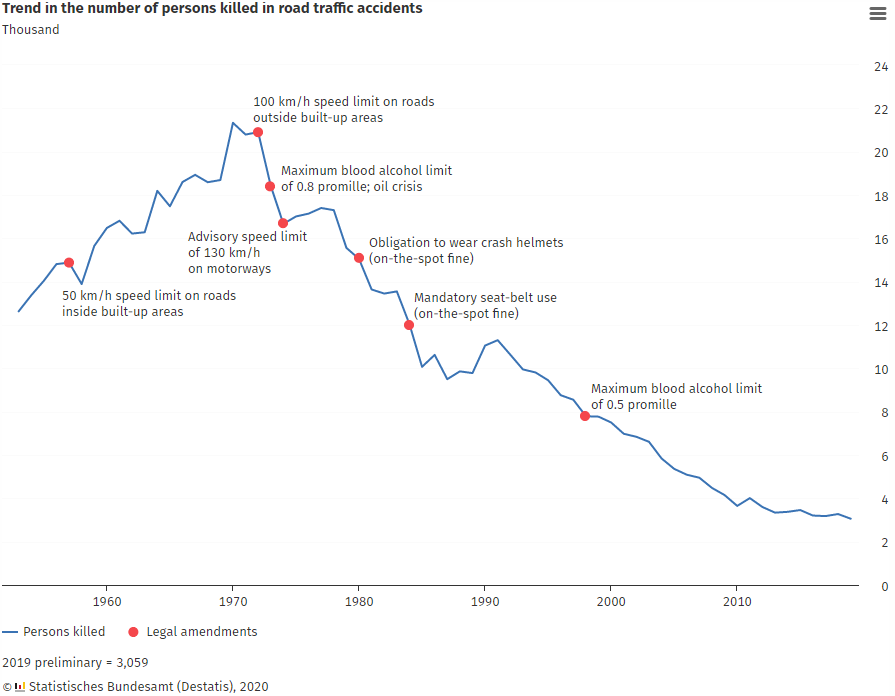
\includegraphics[width=0.9\linewidth]{chapters/chapter6_bruno/Figures/trendV2.png}
  \caption{Car Accident Trend \cite{destatisCar}}
  \label{6fig:trend}
\end{figure}

\noindent
But the decline has stagnated and still leaves around 3000 deaths a year in Germany.
Aside from the measures seen in Figure \ref{6fig:trend}, 
which try to keep accidents from happening, 
there is also another way to potentially save lives.
If the response from medical and police forces to an accident can be improved,
fewer accidents might lead to deaths. 
\\
\newline
This is what this part of the project was about.

